% Options for packages loaded elsewhere
\PassOptionsToPackage{unicode}{hyperref}
\PassOptionsToPackage{hyphens}{url}
%
\documentclass[
  11pt,
  a4paper,oneside]{article}
\usepackage{lmodern}
\usepackage{amssymb,amsmath}
\usepackage{ifxetex,ifluatex}
\ifnum 0\ifxetex 1\fi\ifluatex 1\fi=0 % if pdftex
  \usepackage[T1]{fontenc}
  \usepackage[utf8]{inputenc}
  \usepackage{textcomp} % provide euro and other symbols
\else % if luatex or xetex
  \usepackage{unicode-math}
  \defaultfontfeatures{Scale=MatchLowercase}
  \defaultfontfeatures[\rmfamily]{Ligatures=TeX,Scale=1}
\fi
% Use upquote if available, for straight quotes in verbatim environments
\IfFileExists{upquote.sty}{\usepackage{upquote}}{}
\IfFileExists{microtype.sty}{% use microtype if available
  \usepackage[]{microtype}
  \UseMicrotypeSet[protrusion]{basicmath} % disable protrusion for tt fonts
}{}
\makeatletter
\@ifundefined{KOMAClassName}{% if non-KOMA class
  \IfFileExists{parskip.sty}{%
    \usepackage{parskip}
  }{% else
    \setlength{\parindent}{0pt}
    \setlength{\parskip}{6pt plus 2pt minus 1pt}}
}{% if KOMA class
  \KOMAoptions{parskip=half}}
\makeatother
\usepackage{xcolor}
\IfFileExists{xurl.sty}{\usepackage{xurl}}{} % add URL line breaks if available
\IfFileExists{bookmark.sty}{\usepackage{bookmark}}{\usepackage{hyperref}}
\hypersetup{
  pdftitle={Long-term Changes Surface Solar Shortwave Irradiance at Thessaloniki, Greece under clear- and all-sky conditions},
  pdfauthor={Natsis Athanasios; Alkiviadis Bais; Charikleia Meleti; Kleareti Tourpali},
  hidelinks,
  pdfcreator={LaTeX via pandoc}}
\urlstyle{same} % disable monospaced font for URLs
\usepackage[left=0.5in,right=0.5in,top=0.5in,bottom=0.5in]{geometry}
\usepackage{longtable,booktabs}
% Correct order of tables after \paragraph or \subparagraph
\usepackage{etoolbox}
\makeatletter
\patchcmd\longtable{\par}{\if@noskipsec\mbox{}\fi\par}{}{}
\makeatother
% Allow footnotes in longtable head/foot
\IfFileExists{footnotehyper.sty}{\usepackage{footnotehyper}}{\usepackage{footnote}}
\makesavenoteenv{longtable}
\usepackage{graphicx}
\makeatletter
\def\maxwidth{\ifdim\Gin@nat@width>\linewidth\linewidth\else\Gin@nat@width\fi}
\def\maxheight{\ifdim\Gin@nat@height>\textheight\textheight\else\Gin@nat@height\fi}
\makeatother
% Scale images if necessary, so that they will not overflow the page
% margins by default, and it is still possible to overwrite the defaults
% using explicit options in \includegraphics[width, height, ...]{}
\setkeys{Gin}{width=\maxwidth,height=\maxheight,keepaspectratio}
% Set default figure placement to htbp
\makeatletter
\def\fps@figure{htbp}
\makeatother
\setlength{\emergencystretch}{3em} % prevent overfull lines
\providecommand{\tightlist}{%
  \setlength{\itemsep}{0pt}\setlength{\parskip}{0pt}}
\setcounter{secnumdepth}{-\maxdimen} % remove section numbering
\usepackage{caption}
\usepackage{placeins}
\captionsetup{font=small}
\usepackage{multicol}
\setlength{\columnsep}{1cm}
\newlength{\cslhangindent}
\setlength{\cslhangindent}{1.5em}
\newenvironment{cslreferences}%
  {\setlength{\parindent}{0pt}%
  \everypar{\setlength{\hangindent}{\cslhangindent}}\ignorespaces}%
  {\par}

\title{Long-term Changes Surface Solar Shortwave Irradiance at Thessaloniki, Greece under clear- and all-sky conditions}
\author{Natsis Athanasios\footnote{Laboratory of Atmospheric Physics, AUTH, \href{mailto:natsisthanasis@gmail.com}{\nolinkurl{natsisthanasis@gmail.com}}} \and Alkiviadis Bais\footnote{Laboratory of Atmospheric Physics, AUTH.} \and Charikleia Meleti\footnote{Laboratory of Atmospheric Physics, AUTH.} \and Kleareti Tourpali\footnote{Laboratory of Atmospheric Physics, AUTH.}}
\date{2022-10-14}

\begin{document}
\maketitle

\hypertarget{abstract}{%
\subsection{Abstract}\label{abstract}}

Measurements of downward shortwave solar irradiance (GHI) are performed at Thessaloniki since 1993 with a Kipp \& Zonen CM-21 pyranometer. Data are recorded as 1 min means and are quality controlled by adopting the procedure proposed by Long and Shi (2008). The long time series is analysed in order to investigate long- and short-term changes caused by changes in atmospheric composition over the site. The overall increasing trend in daily solar irradiation under all-sky conditions of 0.33\% per year reported for the period 1993--2012 (Bais et al. 2013) is reconfirmed, although a stronger trend is calculated for the last decade of the data series.

An iterative optimization method has been employed to tune the clear-sky detection algorithm of Reno and Hansen (2016) to the local conditions, in order to identify the cloud-free cases. A few simple global radiation models have been tested and adjustment factors for each model have been determined which match best the measured values.

Linear trends have been calculated for the entire period and different seasons for both clear- and all-sky conditions, in an attempt to attribute the long-term variability to variations in atmospheric water vapor and aerosols. Ancillary information from a collocated Cimel sun-photometer (since 2004), and a pyrheliometer (since 2016) are used to verify the effects of water vapor and aerosols on clear-sky irradiance. Finally, data under cloudy conditions are analysed to uncover potential effects from changes in cloudiness that have occurred over the period or record. References

\hypertarget{introduction}{%
\subsection{Introduction}\label{introduction}}

Radiation clouds trends

\hypertarget{methodology}{%
\subsection{Methodology}\label{methodology}}

Due to larger measurement uncertainty near the horizon, we exclude all measurements with SZA greater than \(85^\circ\). Moreover, due to some obstructions around the site (hills and buildings), we remove data with Azimuth angle between \(35^\circ\) and \(120^\circ\) and SZA greater than \(80^\circ\). As, at those cases the Sun, was not visible by the instruments.

We aggregate the 1-minute values of GHI, to daily mean, for all the days in the data set. Similar, for all the days, with the same day of year number (doy), in order to create the mean annual cycle of the whole data set. Days with less than 50 data point were rejected. By matching the aggregated data series by doy, we calculate the relative seasonal anomaly, as the difference from the climatological mean of each matching day. The same process was applied for the the whole data, that represents the all sky conditions and for a subset of data characterized as clear sky conditions. We calculate the trends of GHI, for those data-sets, by implemented a linear fit regression.

\hypertarget{results-and-discussion}{%
\subsection{Results and discussion}\label{results-and-discussion}}

The trends

Some aspects we have to study is the seasonality of the above finds remove the sza dependence in order to see some local phenomena of the site

\begin{figure}[!h]

{\centering 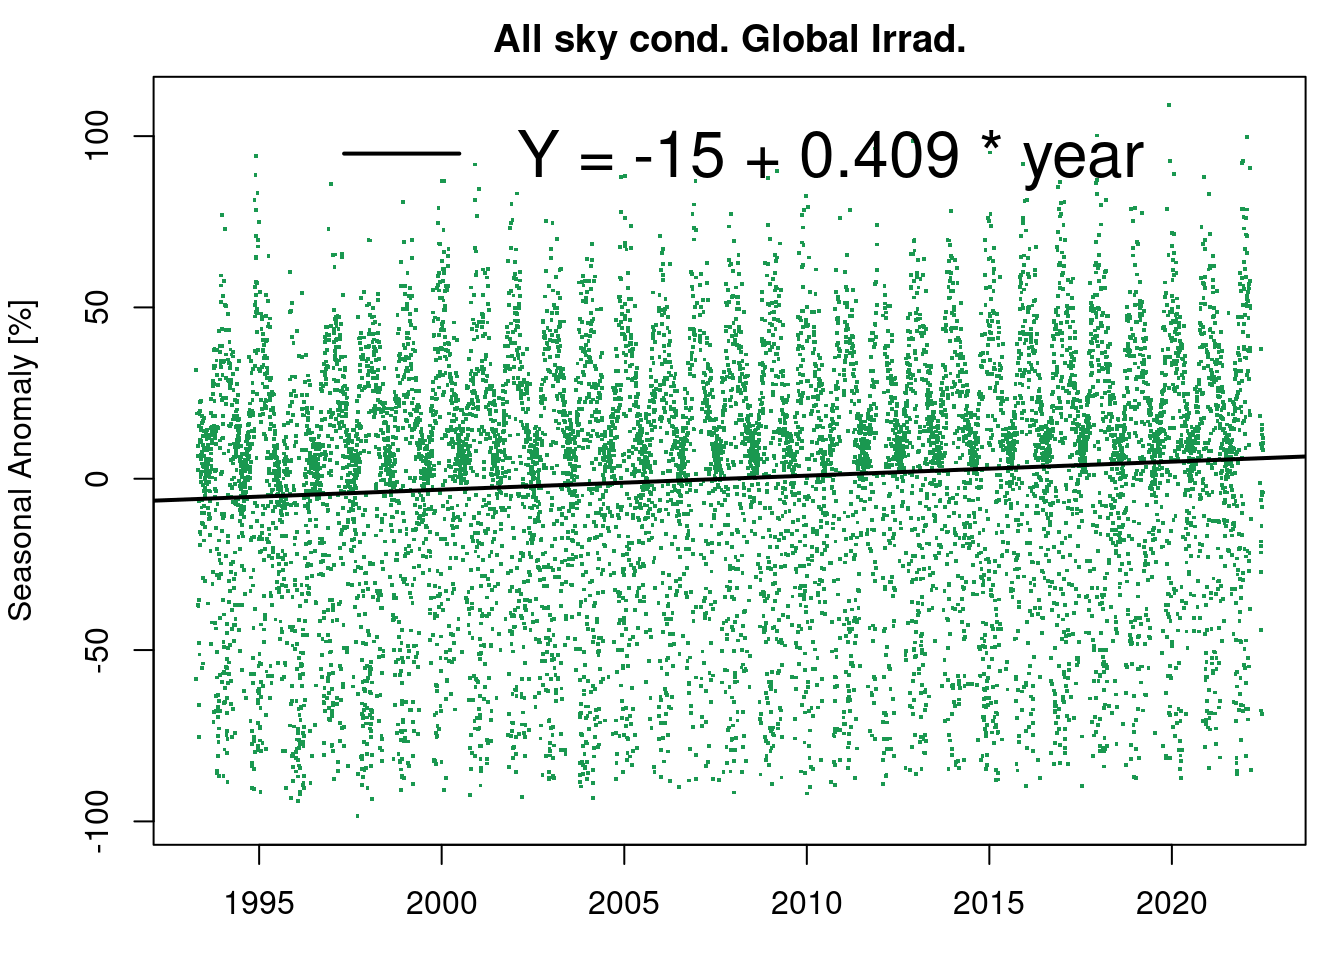
\includegraphics[width=0.6\linewidth]{./figures/longtermtrendsALL-4} 

}

\caption{tracker}\label{fig:alltrend}
\end{figure}

\begin{figure}[!h]

{\centering 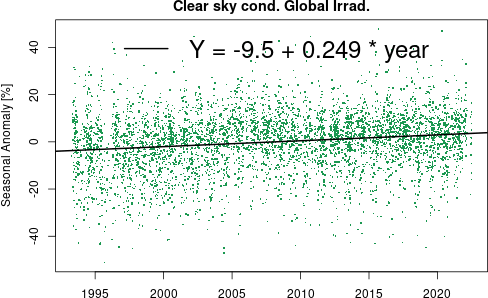
\includegraphics[width=0.6\linewidth]{./figures/longtermtrendsCS-4} 

}

\caption{tracker}\label{fig:cleartrend}
\end{figure}

\begin{longtable}[]{@{}ccccc@{}}
\caption{Trens by season of the year, for clear and all sky conditions.}\tabularnewline
\toprule
\begin{minipage}[b]{0.19\columnwidth}\centering
~\strut
\end{minipage} & \begin{minipage}[b]{0.11\columnwidth}\centering
Winter\strut
\end{minipage} & \begin{minipage}[b]{0.11\columnwidth}\centering
Spring\strut
\end{minipage} & \begin{minipage}[b]{0.11\columnwidth}\centering
Summer\strut
\end{minipage} & \begin{minipage}[b]{0.11\columnwidth}\centering
Automn\strut
\end{minipage}\tabularnewline
\midrule
\endfirsthead
\toprule
\begin{minipage}[b]{0.19\columnwidth}\centering
~\strut
\end{minipage} & \begin{minipage}[b]{0.11\columnwidth}\centering
Winter\strut
\end{minipage} & \begin{minipage}[b]{0.11\columnwidth}\centering
Spring\strut
\end{minipage} & \begin{minipage}[b]{0.11\columnwidth}\centering
Summer\strut
\end{minipage} & \begin{minipage}[b]{0.11\columnwidth}\centering
Automn\strut
\end{minipage}\tabularnewline
\midrule
\endhead
\begin{minipage}[t]{0.19\columnwidth}\centering
\textbf{All Sky}\strut
\end{minipage} & \begin{minipage}[t]{0.11\columnwidth}\centering
0.812\strut
\end{minipage} & \begin{minipage}[t]{0.11\columnwidth}\centering
0.282\strut
\end{minipage} & \begin{minipage}[t]{0.11\columnwidth}\centering
0.183\strut
\end{minipage} & \begin{minipage}[t]{0.11\columnwidth}\centering
0.495\strut
\end{minipage}\tabularnewline
\begin{minipage}[t]{0.19\columnwidth}\centering
\textbf{Clear Sky}\strut
\end{minipage} & \begin{minipage}[t]{0.11\columnwidth}\centering
0.658\strut
\end{minipage} & \begin{minipage}[t]{0.11\columnwidth}\centering
0.38\strut
\end{minipage} & \begin{minipage}[t]{0.11\columnwidth}\centering
0.219\strut
\end{minipage} & \begin{minipage}[t]{0.11\columnwidth}\centering
0.409\strut
\end{minipage}\tabularnewline
\bottomrule
\end{longtable}

~ ~

\hypertarget{refs}{}
\begin{cslreferences}
\leavevmode\hypertarget{ref-Bais2013}{}%
Bais, A. F., T. Drosoglou, C. Meleti, K. Tourpali, and N. Kouremeti. 2013. ``Changes in surface shortwave solar irradiance from 1993 to 2011 at Thessaloniki (Greece).'' \emph{International Journal of Climatology} 33 (13): 2871--6. \url{https://doi.org/10.1002/joc.3636}.

\leavevmode\hypertarget{ref-long_automated_2008}{}%
Long, C. N., and Y. Shi. 2008. ``An Automated Quality Assessment and Control Algorithm for Surface Radiation Measurements.'' \emph{The Open Atmospheric Science Journal}, 23--37.

\leavevmode\hypertarget{ref-Reno2016}{}%
Reno, Matthew J., and Clifford W. Hansen. 2016. ``Identification of periods of clear sky irradiance in time series of GHI measurements.'' \emph{Renewable Energy} 90: 520--31. \url{https://doi.org/10.1016/j.renene.2015.12.031}.
\end{cslreferences}

\end{document}
